\documentclass[12pt]{book}
\usepackage{graphicx}
\usepackage{wrapfig}
\usepackage{caption}
\usepackage{floatrow}
\usepackage{array}
\usepackage{tabularx}

\graphicspath{{images/}}

\title{The Elder Scrolls Tabletop Roleplaying Game Player's Handbook}
\author{William Taylor Cook and Pascalle Audrey Nelson}

\begin{document}

\maketitle

Note: This game is a non-profit fan production intended to turn the complex and storied Elder Scrolls setting into a playable pencil-and-paper RPG. Elder Scrolls and all products under its name are owned by Bethesda Softworks and Bethesda Game Studios. We do not intend to profit off of this in any way. Please support the creators by buying their games and products.\\~\\
By participating in our game as a playtester, you agree to the following terms:

1)	You will not sell any portion of this game under any circumstances.

2)	You acknowledge that any rules and game mechanics may be subject to change by the authors in the service of better gameplay.

3)	You agree to help foster an inclusive, respectful atmosphere for all players. While we trust you all to do this, it bears repeating.\\~\\
In return, we promise the following to you:

1)	Our top priority is and always will be the creation of a satisfying gameplay experience.

2)	We will attempt to implement game changes in an unobtrusive way whenever possible.

3)	We will treat players with respect both out-of-character and in the way we create our narrative (even if player characters may not be respected).

4)	We encourage you to voice your concerns in any way you feel comfortable and will listen to your feedback.\\~\\
We hope you enjoy our game!
\newpage

\section*{About the game}

Elder Scrolls is a vast, intricate fantasy setting. Attempting to compile relevant information here would be an effort in futility without a specific time and place in mind, and these rules are easily applicable to any location throughout much of the Second, Third and early Fourth Eras. The game is largely based on the game mechanics of Elder Scrolls IV: Oblivion and Elder Scrolls III: Morrowind. Some modification would be necessary to make it function more like Elder Scrolls V and set it later in the Fourth Era, but it is possible if you were inclined to do so. For now, please refer to online sources for lore information. In particular, the Unofficial Elder Scrolls Project is a comprehensive and accurate source for information about all things Elder Scrolls. Much of the material here is taken from UESP --- a benefit of this being a not-for-profit fan creation.

Playing this game is a little calculation heavy because of the percentage-based formulas. For example, glass armor reduces incoming physical damage by 35\%. Can you calculate 65\% of a given number easily in your head? It's much easier to use a calculator for these things, so it would be a good idea to have one on hand. Besides that, the formulas are designed to be simple as long as you know what numbers to look at. If they wind up bogging down gameplay too much, they might be changed.

In addition to a calculator, you will need four-sided dice, six-sided dice, eight-sided dice, ten-sided dice and a percentile die. This system primarily relies on percentile-based rolls, not unlike Chaosium's Basic Role-Playing system. To veterans of BRP, your skills and attributes may seem low at first, but you will have the chance to improve them significantly every time you gain a level. The following chapters will tell you how to make a character and play the game.
\newpage
\noindent
\chapter{Character Creation}

Creating a character in the Elder Scrolls Tabletop RPG is a multi-step process with many options for customization. You can choose from 10 races, each with different attributes and traits. You also choose the astrological sign under which your character was born, granting further bonuses. On top of that, there are also 21 skills and 21 classes --- you can even make your own custom class! The choices can seem overwhelming, so let's take this one step at a time.\\

\noindent
\textit{What do all the numbers mean?}

As you create your character, you will assign numbers that represent your character's physical and mental abilities. These numbers are called \textit{attributes,} and they come in two kinds: primary and derived. Primary attributes have an indirect effect on your character, and they are largely determined by your race and birthsign. They are as follows:
\begin{itemize}
	\item Strength: Muscle power. Determines your melee damage bonus.
	\item Intelligence: Mental acuity. Determines your maximum magicka.
	\item Willpower: Strength of will. Determines your magicka regeneration rate.
	\item Agility: Coordination. Determines your ranged damage bonus.
	\item Speed: Rate of bodily movement. Determines your per-round movement speed.
	\item Endurance: Physical health and toughness. Determines your maximum health.
	\item Personality: Charm and beauty. Sets NPCs' initial opinions of you.
\end{itemize}

\noindent
Your derived attributes have a more direct impact on your character.
\begin{itemize}
	\item Health: General condition of your body.
	\item Magicka: Stored magical energy.
	\item Stamina: Ability to endure physical exertion.
	\item Magicka Regeneration Rate: How quickly your magicka recovers.
	\item Stamina Regeneration Rate: How quickly your stamina recovers.
	\item Movement: Your per-round rate of movement.
	\item Damage Bonus: The damage you add to attacks.
\end{itemize}
The Luck attribute from Oblivion is not used, for simplicity. Now that you understand attributes, it is time to start building your character.\\

\section{Choose a Race.}
There are ten playable races which represent the ten mainstream cultures of Tamriel. Each comes with a starting set of attributes as well as skill bonuses and special traits or powers. Each race is listed here along with a picture, description, and stats.\\

\subsection{Altmer (High Elf)}
\begin{wrapfigure}{L}{0.35\textwidth}
	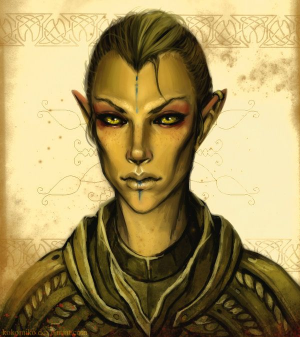
\includegraphics[width=\textwidth]{Altmer.png}
\end{wrapfigure}

The Altmer, or self-titled "Cultured People", are a tall, golden-skinned race, hailing from Summerset Isle. They are also known as High Elves by the denizens of Tamriel. In the Empire, "High" is often understood to mean proud or snobbish, and as the Altmer generally personify these characteristics, the "lesser races" generally resent them. Altmer live two to three times as long as humans; with a 200-year-old Altmer being old and a 300-year-old Altmer being very, very old. Altmer consider themselves to be the most civilized culture of Tamriel; the common tongue of the continent is based on Altmer speech and writing, and most of the Empire's arts, crafts, laws, and sciences are derived from Altmer traditions. They usually have golden, green, or amber eyes.

The Altmer are the most strongly gifted in the arcane arts of all the races, and they are very resistant to diseases. However, they are also somewhat vulnerable to magicka, fire, frost, and shock, which makes them very weak against their strongest point --- magic. They are among the longest living and most intelligent races of Tamriel, and they often become powerful magic users due to both their magical affinity and the many years they may devote to their studies.

Altmer begin the game with the following attributes:

\begin{center}
\begin{tabular}{|c|c|c|c|c|c|c|}
\hline
STR & INT & WIL & AGI & SPD & END & PER\\ \hline
30 & 50 & 40 & 40 & 35 & 35 & 40\\ \hline
\end{tabular}
\end{center}

They also get the following skill bonuses: +5 Alchemy, +10 Alteration, +5 Conjuration, +10 Destruction, +5 Illusion, +10 Mysticism.

Altmer have a permanent +100 bonus to max magicka and a 75\% resistance to disease; however, they have a 25\% vulnerability to fire, frost and shock damage.\\

\subsection{Argonian}
\begin{wrapfigure}{L}{0.4\textwidth}
	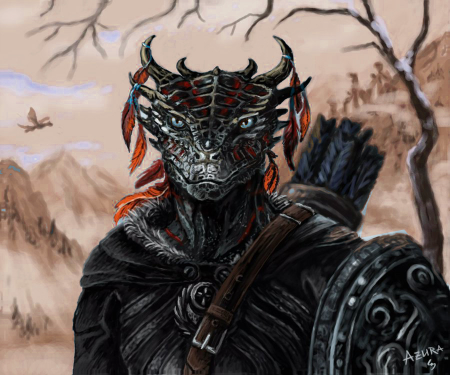
\includegraphics[width=\textwidth]{Argonian.png}
\end{wrapfigure}

Argonians (in their native tongue of Jel they call themselves the Saxhleel, or People of the Root) are the reptilian natives of Black Marsh, a vast swampland province in southeastern Tamriel. The other races often prefer to refer to them as 'lizards' or the 'Lizard Folk' instead, especially when meaning to be derogative. They are known as the foremost experts in guerrilla warfare throughout the Starry Heart, a reputation brought upon them by defending their borders from enemies for countless centuries. Argonians have a lifespan similar to that of humans. According to the First Era Scholar Brendan the Persistent "the Argonian people have, throughout Tamrielic history, been perhaps the most misunderstood, vilified, and reviled of all the sentient races. Yet, those who have taken the time to experience Argonian culture have gained a greater appreciation for this noble and beautiful people." However, it should be noted that he himself went missing in his final expedition into the deeper swamps of their homeland.

Argonians get the following skill bonuses: +5 Alchemy, +10 Athletics, +5 Blade, +5 Hand-to-Hand, +5 Illusion, +5 Mysticism, +10 Security.

They have a complete immunity to poison and a 75\% resistance to disease. They can breathe underwater and are adept swimmers, suffering no movement penalty or melee attack penalty in water.

Argonians begin the game with the following attributes:

\begin{center}
\begin{tabular}{|c|c|c|c|c|c|c|}
\hline
STR & INT & WIL & AGI & SPD & END & PER\\ \hline
40 & 45 & 35 & 45 & 45 & 30 & 30\\ \hline
\end{tabular}
\end{center}

\subsection{Bosmer}
\begin{wrapfigure}{L}{0.35\textwidth}
	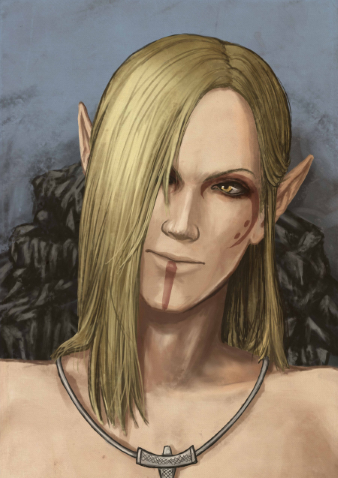
\includegraphics[width=\textwidth]{Bosmer.png}
\end{wrapfigure}

The Bosmer are the Elven clan-folk of Valenwood, a forested province in southwestern Tamriel. In the Empire, they are often referred to as Wood Elves, but Bosmer, Boiche, or the Tree-Sap people is what they call themselves. Bosmer rejected the stiff, formal traditions of Aldmeri high culture, preferring a more romantic, simple existence in harmony with the land and its wild beauty and creatures. They are relatively nimble and quick in body compared to their more "civilized" Altmeri cousins (who often look down upon the Bosmer as unruly and naive). Their agility makes them well-suited as scouts and thieves. However, they are also a quick-witted folk, and many pursue successful careers in scholarly pursuits or trading. Bosmer live two to three times as long as humans; with a 200-year-old Bosmer being old and a 300-year-old Bosmer being very, very old. Though they are considered less influential than some of their Elven brethren, the Bosmer are also relatively prone to producing offspring. As a result, they outnumber all other mer on Tamriel.

The best archers in all of Tamriel, the Bosmer snatch and fire arrows in one continuous motion; they are even rumored to have invented the bow. They have many natural and unique abilities; notably, they can command simple-minded creatures and have a nearly chameleon-like ability to hide in forested areas. Many in the forests of Valenwood follow the tenets of the Green Pact. These "Green Pact Bosmer" are religiously carnivorous and cannibalistic, and do not harm the vegetation of Valenwood, though they are not averse to using wooden or plant-derived products created by others.

Bosmer begin the game with the following attributes:
\begin{center}
\begin{tabular}{|c|c|c|c|c|c|c|}
\hline
STR & INT & WIL & AGI & SPD & END & PER\\ \hline
30 & 40 & 30 & 50 & 50 & 35 & 35\\ \hline
\end{tabular}
\end{center}

They also get the following skill bonuses: +5 Acrobatics, +10 Alchemy, +5 Alteration, +5 Light Armor, +10 Marksman, +10 Sneak.

Bosmer have a 75\% resistance to disease. They get the Beast Tongue power as well, which lets them control lesser animals for 1 minute once a day.\\

\subsection{Breton}
\begin{wrapfigure}{L}{0.3\textwidth}
	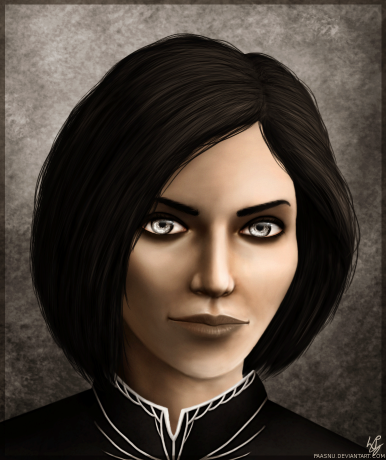
\includegraphics[width=\textwidth]{Breton.png}
\end{wrapfigure}

Bretons are the human descendants of the Aldmeri-Nedic Manmer of the Merethic Era and are now the inhabitants of the province of High Rock. They are united in culture and language, even though they are divided politically, for High Rock is a fractious region. Bretons make up the peasantry, soldiery, and magical elite of the feudal kingdoms that compete for power. Many are capable mages with innate resistance to magicka. They are known for a proficiency in abstract thinking and unique customs. Bretons appear, by and large, much like other pale-skinned humans. They are usually slight of build and not as muscular as Nords or Redguards. Their Elvish ancestry is usually only detectable upon a closer inspection of their eyebrows, ears, or high cheekbones, though many individual Bretons appear to be more Nordic or Imperial than anything else. The great diversity in their appearance is to be expected from their politically fractured society, though their clothes, accents, customs and names are fairly uniform.

Bretons get the following skill bonuses: +5 Alchemy, +5 Alteration, +10 Conjuration, +5 Illusion, +10 Mysticism, +10 Restoration.

They have a natural 50\% resistance to magic and gain a permanent +50 bonus to max magicka. Their Dragon Skin power gives them 50\% physical resistance for 1 minute, once a day.\\

Bretons start the game with the following attributes:
\begin{center}
\begin{tabular}{|c|c|c|c|c|c|c|}
\hline
STR & INT & WIL & AGI & SPD & END & PER\\ \hline
35 & 50 & 50 & 30 & 35 & 30 & 40\\ \hline
\end{tabular}
\end{center}

\subsection{Dunmer}
\begin{wrapfigure}{L}{0.35\textwidth}
	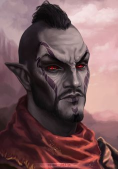
\includegraphics[width=\textwidth]{Dunmer.png}
\end{wrapfigure}

The Dunmer, also known as Dark Elves, are the ash-skinned, typically red-eyed elven peoples of Morrowind. "Dark" is commonly understood as meaning such characteristics as "dark-skinned", "gloomy", "ill-favored by fate" and so on. The Dunmer and their national identity, however, embrace these various connotations with enthusiasm. In the Empire, "Dark Elf" is the common usage, but among their Aldmeri brethren they are called "Dunmer". Their combination of powerful intellects with strong and agile physiques produce superior warriors and sorcerers. On the battlefield, Dunmer are noted for their skill with a balanced integration of the sword, the bow and destruction magic. Dunmer live two to three times as long as humans; with a 200-year-old Dunmer being old and a 300-year-old Dunmer being very, very old. In character, they are grim, aloof, and reserved, as well as distrusting and disdainful of other races.

Dunmer distrust and are treated distrustfully by other races. They are often proud, clannish, ruthless, and cruel, from an outsider's point of view, but greatly value loyalty and family. Young female Dunmer have a reputation for promiscuity in some circles. Despite their powerful skills and strengths, the Dunmer's vengeful nature, age-old conflicts, betrayals, and ill-reputation prevent them from gaining more influence. Those born in their homeland of Morrowind are known to be considerably less friendly than those who grew up in the Imperial tradition.

Dunmer begin the game with the following attributes:
\begin{center}
\begin{tabular}{|c|c|c|c|c|c|c|}
\hline
STR & INT & WIL & AGI & SPD & END & PER\\ \hline
40 & 40 & 30 & 40 & 50 & 35 & 35\\ \hline
\end{tabular}
\end{center}

They also get the following skill bonuses: +5 Athletics, +10 Blade, +5 Blunt, +10 Destruction, +5 Light Armor, +5 Marksman, +5 Mysticism.

Dunmer have a natural 75\% resistance to fire. They can also summon an ancestral spirit to aid them in battle for 1 minute, once a day.\\

\subsection{Imperial}
\begin{wrapfigure}{l}{0.5\textwidth}
	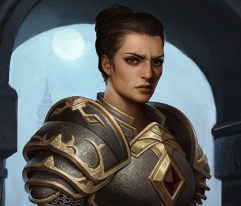
\includegraphics[width=\textwidth]{Imperial.png}
\end{wrapfigure}

Also known as Cyrodiils, Cyrodilics, Cyro-Nordics and Imperial Cyrods, the well-educated and well-spoken Imperials are the natives of the civilized, cosmopolitan province of Cyrodiil. Imperials are also known for the discipline and training of their citizen armies, and their respect for the rule of law. Though physically less imposing than the other races, the Imperials have proved to be shrewd diplomats and traders, and these traits, along with their remarkable skill and training as light infantry, have enabled them to subdue all the other nations and races and erect the monument to peace and prosperity that comprises the Glorious Empire. Their hegemony has waxed and waned throughout the eras, and most historians refer to three distinct Empires, the ends of which each mark a new epoch in Tamrielic history.

Imperials begin the game with the following attributes:
\begin{center}
\begin{tabular}{|c|c|c|c|c|c|c|}
\hline
STR & INT & WIL & AGI & SPD & END & PER\\ \hline
40 & 40 & 35 & 30 & 35 & 40 & 50\\ \hline
\end{tabular}
\end{center}

They also get the following skill bonuses: +5 Blade, +5 Blunt, +5 Hand-to-Hand, +10 Heavy Armor, +10 Mercantile, +10 Speechcraft.

Imperials gain two major powers: Star of the West, which lets them absorb 100 stamina on touch once per day, and Voice of the Emperor, which charms a target for 30 seconds once per day.\\

\subsection{Khajiit}
\begin{wrapfigure}{l}{0.5\textwidth}
	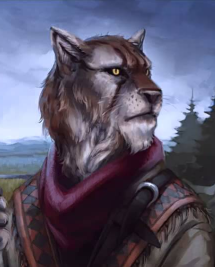
\includegraphics[width=\textwidth]{Khajiit.png}
\end{wrapfigure}

Khajiit are cat-like people who come from Elsweyr, known for high intelligence and agility. These traits make them very good thieves and acrobats, but Khajiit are also fearsome warriors. However, they are rarely known to be mages. Khajiit mostly stay on land, but piracy and skooma trade does draw some to work as sailors.

Khajiit anatomy differs greatly from both men and elves, not only because of their fur, tail, and sometimes toe-walking stance, but also their digestive system and metabolism. Khajiit, Argonians, and Imga are the so-called "beast races" of Tamriel because of these large differences. Khajiit have a lifespan similar to that of humans. There are no well-documented cases of cross-breeding between Khajiit and other races, though there are rumors of such a thing. The foreign appearance and behavior of Khajiit make them common targets of racial discrimination.

Khajiit begin the game with the following attributes:
\begin{center}
\begin{tabular}{|c|c|c|c|c|c|c|}
\hline
STR & INT & WIL & AGI & SPD & END & PER\\ \hline
35 & 40 & 30 & 50 & 40 & 35 & 40\\ \hline
\end{tabular}
\end{center}

They also get the following skill bonuses: +10 Acrobatics, +5 Athletics, +5 Blade, +10 Hand-to-Hand, +5 Light Armor, +5 Security, +5 Sneak.

Khajiit have cat eyes that allow them to see in the dark and claws that boost their unarmed attack damage to 1d4+1+DB. In addition to this, the Eye of Fear power lets them inflict fear for 3 rounds on a single target who can see them, once a day.\\

\subsection{Nord}
\begin{wrapfigure}{l}{0.5\textwidth}
	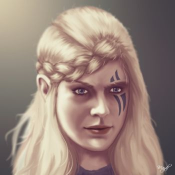
\includegraphics[width=\textwidth]{Nord.png}
\end{wrapfigure}

The Nords are the children of the sky, a race of tall and fair-haired humans from Skyrim who are known for their incredible resistance to cold and magical frost. They are fierce, strong and enthusiastic warriors, and many become renowned warriors, soldiers and mercenaries all over Tamriel. Eager to augment their martial skills beyond the traditional methods of Skyrim, they excel in all manner of warfare, and are known as a militant people by their neighbors. Nords are also natural seamen, and have benefited from nautical trade since their first migrations from Atmora. They captain and crew many merchant fleets, and may be found all along the coasts of Tamriel.

Nords begin the game with the following attributes:
\begin{center}
\begin{tabular}{|c|c|c|c|c|c|c|}
\hline
STR & INT & WIL & AGI & SPD & END & PER\\ \hline
50 & 30 & 35 & 40 & 40 & 45 & 30\\ \hline
\end{tabular}
\end{center}

They also get the following skill bonuses: +5 Armorer, +10 Blade, +5 Block, +10 Blunt, +10 Heavy Armor, +5 Restoration.

Nords have a 50\% resistance to frost damage and can channel Nordic Frost to deal 50 points of frost damage on touch once per day. The Woad power grants them 30\% physical damage reduction for one minute once per day.\\

\subsection{Orc}
\begin{wrapfigure}{l}{0.5\textwidth}
	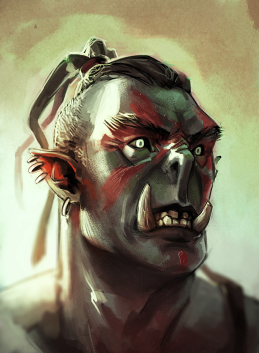
\includegraphics[width=\textwidth]{Orc.png}
\end{wrapfigure}

Orcs, also called Orsimer or "Pariah Folk" in ancient times, are sophisticated, beastlike people of the Wrothgarian Mountains, Dragontail Mountains, Valenwood, and Orsinium (literally translated as "Orc-Town"). They are noted for their unshakable courage in war and their unflinching endurance of hardships. Orcs have elven blood, but are usually considered to be beastfolk. In the past, Orcs have been widely feared and hated by the other nations and races of Tamriel, and were often considered to be goblin-ken. However, they have slowly won acceptance in the Empire, in particular for their distinguished service in the Emperor's Legions. Orc armorers are prized for their craftsmanship, and Orc warriors in heavy armor are among the finest front-line troops in the Empire, and are fearsome when using their berserker rage. Orcs have a lifespan similar to that of humans. Most Imperial citizens regard the Orc society as rough and cruel. The Orcs of the Iliac Bay region have developed their own language, known as Orcish, and have often had their own kingdom, Orsinium.

Orcs begin the game with the following attributes:
\begin{center}
\begin{tabular}{|c|c|c|c|c|c|c|}
\hline
STR & INT & WIL & AGI & SPD & END & PER\\ \hline
45 & 35 & 45 & 35 & 30 & 50 & 30\\ \hline
\end{tabular}
\end{center}

They also get the following skill bonuses: +10 Armorer, +5 Block, +10 Blunt, +5 Hand-to-Hand, +10 Heavy Armor.

Orcs have a natural 25\% resistance to magic. Once a day they may enter a berserk state for 1 minute, which grants the following effects: Fortify Stamina 200, Fortify Health 20, Fortify Strength 50, Drain Agility 100.\\

\subsection{Redguard}
\begin{wrapfigure}{l}{0.5\textwidth}
	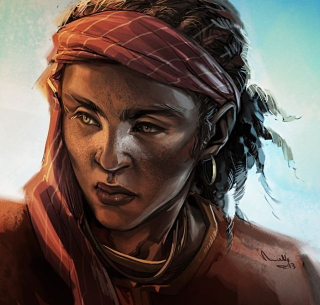
\includegraphics[width=\textwidth]{Redguard.png}
\end{wrapfigure}

Redguards are the most naturally talented warriors in Tamriel. The dark-skinned, wiry-haired people of Hammerfell seem born to battle, though their pride and fierce independence of spirit makes them more suitable as scouts or skirmishers, or as free-ranging heroes and adventurers, than as rank-and-file soldiers. In addition to their cultural affinities for many armor styles and weapons (particularly swords), Redguards are also physically blessed with hardy constitutions, resistance to poison, and quickness of foot. Redguards do not share the same blood as the other human races, and they have no known connection with the ancestral Nordic homeland of Atmora.

Redguards begin the game with the following attributes:
\begin{center}
\begin{tabular}{|c|c|c|c|c|c|c|}
\hline
STR & INT & WIL & AGI & SPD & END & PER\\ \hline
45 & 30 & 30 & 40 & 40 & 50 & 35\\ \hline
\end{tabular}
\end{center}

They also get the following skill bonuses: +10 Athletics, +10 Blade, +10 Blunt, +5 Heavy Armor, +5 Light Armor, +5 Mercantile.

Hardy of constitution, Redguards have a natural 75\% resistance to poison and disease. Once a day, they can have an Adrenaline Rush which grants the following effects for 1 minute: Fortify Agility 50, Fortify Endurance 50, Fortify Speed 50, Fortify Strength 50, Fortify Health 25.\\

Be sure to take note of all your race's skill bonuses and abilities. Skills will be covered in greater detail in the next chapter, so you may wish to come back here once you learn more about them. For now, let's move on.
\section{Choose a Birthsign.}
The people of Tamriel mark their calendars by the passage of constellations overhead. When the sun passes near one, it is that constellation's season. There are thirteen in total: one for each month of the year and then one which seems to wander intermittently, giving it no predictable season. This collection of constellations is known as the Firmament, and many attribute personality traits to the sign under which one was born. The signs of the Firmament are listed here in chronological order; each one grants a certain bonus which may include attribute increases and powers.\\~\\

\begin{figure}[H]
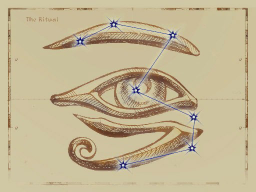
\includegraphics[width=0.6\textwidth]{Ritual.png}
\centering
\caption*{1. The Ritual: The month of Morning Star is marked by the Ritual, a sign denoting a deep connection with the moons and the Divines. Those born under the ritual gain two powers: Mara's Gift (allows them to heal themselves for 200 their health once a day) and Blessed Word (causes undead to flee for 3 rounds for 40 magicka).}
\end{figure}

\begin{figure}[H]
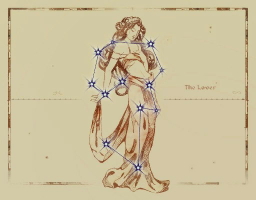
\includegraphics[width=0.6\textwidth]{Lover.png}
\centering
\caption*{2. The Lover: Those born in the month of Sun's Dawn under the Lover are said to be passionate and graceful. The Lover bestows the Lover's Kiss power, which allows the user to paralyze a target on touch for one round at the cost of 120 stamina damage.}
\end{figure}

\begin{figure}[H]
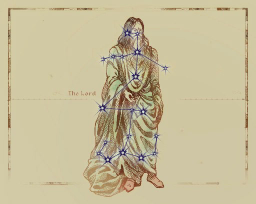
\includegraphics[width=0.6\textwidth]{Lord.png}
\centering
\caption*{3. The Lord: The Lord marks the month of First Seed, where he oversees all the planting in Tamriel. Those born under the Lord are said to be healthier than usual and are granted the Blood of the North power, allowing them to heal 45 health per round for 2 rounds at the cost of 50 magicka. However, they are also cursed with Troll's Blood, giving them a 25\% weakness to fire.}
\end{figure}

\begin{figure}[H]
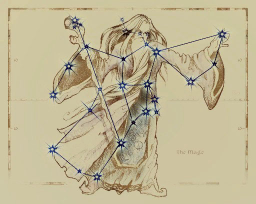
\includegraphics[width=0.6\textwidth]{Mage.png}
\centering
\caption*{4. The Mage: One of the three guardian signs, the Mage marks the month of Rain's Hand, when magicka was first used by humans. Those born under the Mage are particularly gifted in the arcane arts and gain a permanent +50 bonus to maximum magicka.}
\end{figure}

\begin{figure}[H]
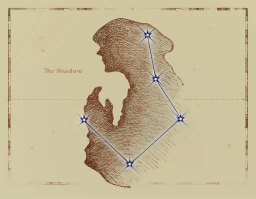
\includegraphics[width=0.6\textwidth]{Shadow.png}
\centering
\caption*{5. The Shadow: The Shadow's season is the month of Second Seed. This sign grants those born under it the power of Moonshadow, which lets them turn invisible for one minute, once a day.}
\end{figure}

\begin{figure}[H]
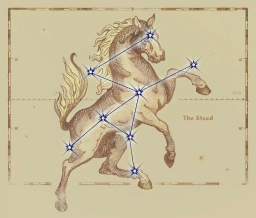
\includegraphics[width=0.6\textwidth]{Steed.png}
\centering
\caption*{6. The Steed: Those born in the month of Mid Year under the sign of the Steed are impatient, always hurrying from place to place and restless whenever they have to wait. They gain a permanent +20 bonus to their Speed attribute.}
\end{figure}

\begin{figure}[H]
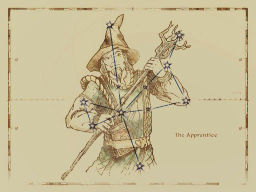
\includegraphics[width=0.6\textwidth]{Apprentice.png}
\centering
\caption*{7. The Apprentice: The month of Sun's Height is the season of the Apprentice. Those born under this sign are especially gifted with magic and gain a permanent +100 to max magicka; however, they also gain a permanent 100\% vulnerability to magic.}
\end{figure}

\begin{figure}[H]
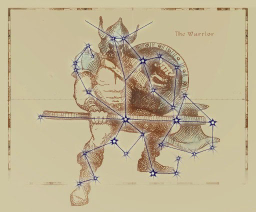
\includegraphics[width=0.6\textwidth]{Warrior.png}
\centering
\caption*{8. The Warrior: The Warrior is another of the guardian signs. It marks the month of Last Seed and is said to grant those born in this month skill with weapons of all kinds as well as a short temper. This sign grants a permanent +10 bonus to both Endurance and Strength.}
\end{figure}

\begin{figure}[H]
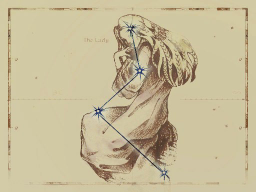
\includegraphics[width=0.6\textwidth]{Lady.png}
\centering
\caption*{9. The Lady: The Lady presides graciously over the month of Heartfire. Those born under this sign are said to be kind and tolerant, and they gain a permanent +10 bonus to both Willpower and Endurance.}
\end{figure}

\begin{figure}[H]
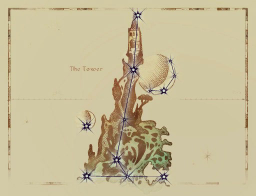
\includegraphics[width=0.6\textwidth]{Tower.png}
\centering
\caption*{10. The Tower: The Tower is a birthsign of great fortune, and those born under it are said to find treasure in one way or another. The Tower grants two powers: Tower Key (open a lock of average level or lower for free once a day) and Tower Warden (5\% chance to reflect incoming damage back to the target for 1 minute).}
\end{figure}

\begin{figure}[H]
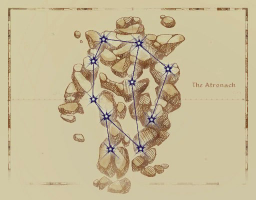
\includegraphics[width=0.5\textwidth]{Atronach.png}
\centering
\caption*{11. The Atronach: A sign representing elemental beings from Oblivion, the Atronach is both a blessing and a curse to aspiring mages. Those born under the Atronach gain a permanent +150 bonus to maximum magicka and have a 50\% chance to absorb spells targeting them (meaning they have no effect and you gain the magicka used to cast the spell). However, they cannot regenerate magicka on their own.}
\end{figure}

\begin{figure}[H]
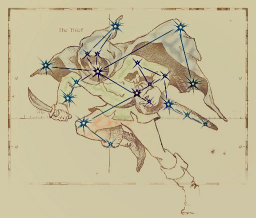
\includegraphics[width=0.5\textwidth]{Thief.png}
\centering
\caption*{12. The Thief: The final month of the year is Evening Star, and it is marked by the guardian sign of the Thief. Those born under the Thief are not necessarily thieves; instead, they are prone to risky lifestyles and rarely come to harm due to their natural luck. They receive a permanent +10 bonus to both Speed and Agility.}
\end{figure}

\begin{figure}[H]
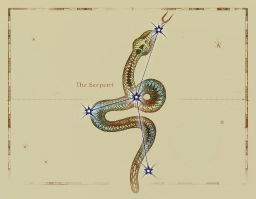
\includegraphics[width=0.5\textwidth]{Serpent.png}
\centering
\caption*{13. The Serpent: There are no common characteristics amongst those born under the Serpent, but they are said to be the most blessed and the most cursed. The Serpent grants the power of Serpent Spell, which has the following effects: the user may touch a target and damage them for 30 health per round for 2 rounds; whether or not a target is touched, the user is cured of poison, all magical effects of Expert level or lower are dispelled, and 100 stamina points are lost. This power may be used once per day.}
\end{figure}

\newpage
\section{Choose a class.}
There are a grand total of 21 classes in the Elder Scrolls Tabletop RPG, each with a unique combination of favored skills and attributes. You may wish to become more acquainted with what the skills mean in order to make an informed decision about which class you choose.

A class consists of 4 components:
\begin{enumerate}
	\item A name.
	\item A specialization (combat, magic or stealth).
	\item Two favored primary attributes.
	\item Seven major skills.
\end{enumerate}

All skills grouped under the chosen specialization get a +5 bonus. The two favored attributes gain a +5 bonus as well. The seven major skills gain a +20 bonus; the remaining 14 skills are defined as minor skills. If you wish to create a custom class, simply choose the four components on your own. You should look over the 21 existing classes, however --- odds are you'll find multiple appealing choices.\\

\begin{figure}[H]
\floatbox[{\capbeside\thisfloatsetup{capbesideposition={right,top},capbesidewidth=0.5\textwidth}}]{figure}[\FBwidth]
{\caption*{Acrobat\\

The kind of person that uses agility and endurance to their advantage. Unafraid of jumping long distances.\\

Specialization: Stealth.\\

Attributes: Agility, Endurance.\\

Skills: Acrobatics, Blade, Block, Marksman, Security, Sneak, Speechcraft.}\label{fig:test}}
{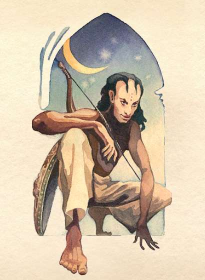
\includegraphics[width=0.45\textwidth]{Acrobat.png}}
\end{figure}

\begin{figure}[H]
\floatbox[{\capbeside\thisfloatsetup{capbesideposition={right,top},capbesidewidth=0.5\textwidth}}]{figure}[\FBwidth]
{\caption*{Agent\\

Charming when they can be seen, and nearly invisible when in shadow.\\

Specialization: Stealth.\\

Attributes: Agility, Personality.\\

Skills: Acrobatics, Illusion, Marksman, Mercantile, Security, Sneak, Speechcraft.}\label{fig:test}}
{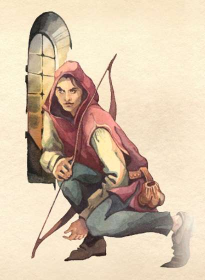
\includegraphics[width=0.45\textwidth]{Agent.png}}
\end{figure}

\begin{figure}[H]
\floatbox[{\capbeside\thisfloatsetup{capbesideposition={right,top},capbesidewidth=0.5\textwidth}}]{figure}[\FBwidth]
{\caption*{Archer\\

A marksman, adept at combat at great distances. Able to take down most foes before they have a chance to draw sword.\\

Specialization: Combat.\\

Attributes: Agility, Strength.\\

Skills: Armorer, Blade, Blunt, Hand-to-Hand, Light Armor, Marksman, Sneak.}\label{fig:test}}
{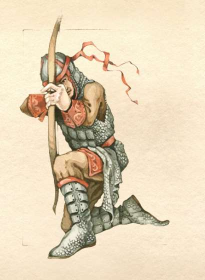
\includegraphics[width=0.45\textwidth]{Archer.png}}
\end{figure}

\begin{figure}[H]
\floatbox[{\capbeside\thisfloatsetup{capbesideposition={right,top},capbesidewidth=0.5\textwidth}}]{figure}[\FBwidth]
{\caption*{Assassin\\

Nimble and quiet, they move in darkness to strike at the unsuspecting. Locks hold no doors shut for them.\\

Specialization: Stealth.\\

Attributes: Intelligence, Speed.\\

Skills: Acrobatics, Alchemy, Blade, Light Armor, Marksman, Security, Sneak.}\label{fig:test}}
{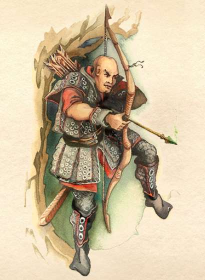
\includegraphics[width=0.45\textwidth]{Assassin.png}}
\end{figure}

\begin{figure}[H]
\floatbox[{\capbeside\thisfloatsetup{capbesideposition={right,top},capbesidewidth=0.5\textwidth}}]{figure}[\FBwidth]
{\caption*{Barbarian\\

Fearsome brutes who inspire fear and dread in the hearts of their enemies. Like a storm, swift and powerful. Finding little use for heavy armor, they rely on smashing their foes into the ground.\\

Specialization: Combat.\\

Attributes: Speed, Strength.\\

Skills: Armorer, Athletics, Blade, Block, Blunt, Hand-to-Hand, Light Armor.}\label{fig:test}}
{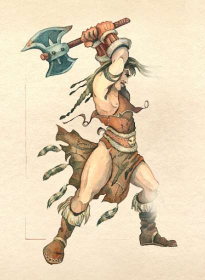
\includegraphics[width=0.45\textwidth]{Barbarian.png}}
\end{figure}

\begin{figure}[H]
\floatbox[{\capbeside\thisfloatsetup{capbesideposition={right,top},capbesidewidth=0.5\textwidth}}]{figure}[\FBwidth]
{\caption*{Bard\\

Intelligent and personable, they prefer to accomplish tasks with their words first, and sword second.\\

Specialization: Stealth.\\

Attributes: Intelligence, Personality.\\

Skills: Alchemy, Blade, Block, Illusion, Light Armor, Mercantile, Speechcraft.}\label{fig:test}}
{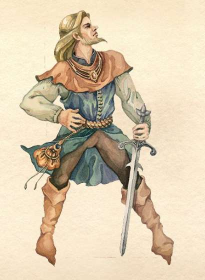
\includegraphics[width=0.45\textwidth]{Bard.png}}
\end{figure}

\begin{figure}[H]
\floatbox[{\capbeside\thisfloatsetup{capbesideposition={right,top},capbesidewidth=0.5\textwidth}}]{figure}[\FBwidth]
{\caption*{Battlemage\\

Able to resolve most conflicts with either spell or sword. They are a deadly mix of scholar and soldier.\\

Specialization: Magic.\\

Attributes: Intelligence, Strength.\\

Skills: Alchemy, Alteration, Blade, Blunt, Conjuration, Destruction, Mysticism.}\label{fig:test}}
{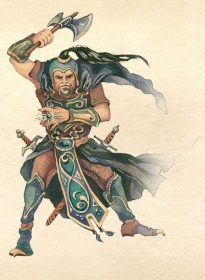
\includegraphics[width=0.45\textwidth]{Battlemage.png}}
\end{figure}

\begin{figure}[H]
\floatbox[{\capbeside\thisfloatsetup{capbesideposition={right,top},capbesidewidth=0.5\textwidth}}]{figure}[\FBwidth]
{\caption*{Crusader\\

A combatant who wields the power of brute strength and medicinal knowledge. Cheating death after every fight, they rely on their keen knowledge of restoration to fight yet again.\\

Specialization: Combat.\\

Attributes: Strength, Willpower.\\

Skills: Athletics, Blade, Blunt, Destruction, Hand-to-Hand, Heavy Armor, Restoration.}\label{fig:test}}
{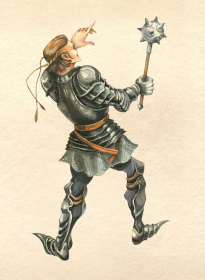
\includegraphics[width=0.45\textwidth]{Crusader.png}}
\end{figure}

\begin{figure}[H]
\floatbox[{\capbeside\thisfloatsetup{capbesideposition={right,top},capbesidewidth=0.5\textwidth}}]{figure}[\FBwidth]
{\caption*{Healer\\

Fighters of poison and illness. The ancient art of restoration is their ally, and the deadly art of destruction is their weapon.\\

Specialization: Magic.\\

Attributes: Personality, Willpower.\\

Skills: Alchemy, Alteration, Destruction, Illusion, Mercantile, Restoration, Speechcraft.}\label{fig:test}}
{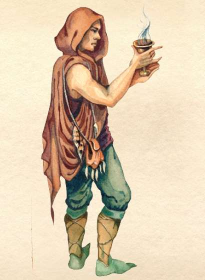
\includegraphics[width=0.45\textwidth]{Healer.png}}
\end{figure}

\begin{figure}[H]
\floatbox[{\capbeside\thisfloatsetup{capbesideposition={right,top},capbesidewidth=0.5\textwidth}}]{figure}[\FBwidth]
{\caption*{Knight\\

The most noble of all combatants. Strong in body and in character.\\

Specialization: Combat.\\

Attributes: Personality, Strength.\\

Skills: Blade, Block, Blunt, Hand-to-Hand, Heavy Armor, Illusion, Speechcraft.}\label{fig:test}}
{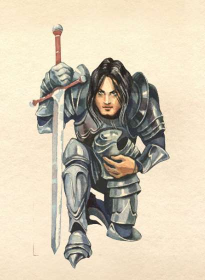
\includegraphics[width=0.45\textwidth]{Knight.png}}
\end{figure}

\begin{figure}[H]
\floatbox[{\capbeside\thisfloatsetup{capbesideposition={right,top},capbesidewidth=0.5\textwidth}}]{figure}[\FBwidth]
{\caption*{Mage\\

Preferring to use their extensive knowledge of all things magical, they wield a might more powerful than the sharpest blade.\\

Specialization: Magic.\\

Attributes: Intelligence, Willpower.\\

Skills: Alchemy, Alteration, Conjuration, Destruction, Illusion, Mysticism, Restoration.}\label{fig:test}}
{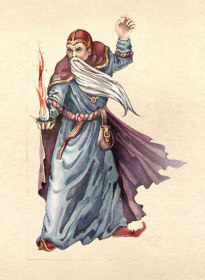
\includegraphics[width=0.45\textwidth]{Mageclass.png}}
\end{figure}

\begin{figure}[H]
\floatbox[{\capbeside\thisfloatsetup{capbesideposition={right,top},capbesidewidth=0.5\textwidth}}]{figure}[\FBwidth]
{\caption*{Monk\\

Quick and cunning with the empty hand, they are strong in spirit. They prefer to solve conflict by arrow or by fist.\\

Specialization: Stealth.\\

Attributes: Agility, Willpower.\\

Skills: Acrobatics, Alteration, Athletics, Hand-to-Hand, Marksman, Security, Sneak.}\label{fig:test}}
{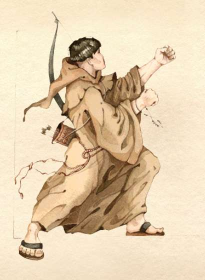
\includegraphics[width=0.45\textwidth]{Monk.png}}
\end{figure}

\begin{figure}[H]
\floatbox[{\capbeside\thisfloatsetup{capbesideposition={right,top},capbesidewidth=0.5\textwidth}}]{figure}[\FBwidth]
{\caption*{Nightblade\\

Spell and shadow are their friends. By darkness they move with haste, casting magic to benefit their circumstances.\\

Specialization: Magic.\\

Attributes: Speed, Willpower.\\

Skills: Acrobatics, Alteration, Athletics, Blade, Destruction, Light Armor, Restoration.}\label{fig:test}}
{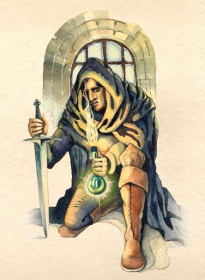
\includegraphics[width=0.45\textwidth]{Nightblade.png}}
\end{figure}

\begin{figure}[H]
\floatbox[{\capbeside\thisfloatsetup{capbesideposition={right,top},capbesidewidth=0.5\textwidth}}]{figure}[\FBwidth]
{\caption*{Pilgrim\\

Hearty folk, well-versed in the tomes of old. They profit in life by bartering in the market, or by persuading the weak-minded.\\

Specialization: Stealth.\\

Attributes: Endurance, Personality.\\

Skills: Armorer, Block, Blunt, Light Armor, Mercantile, Security, Speechcraft.}\label{fig:test}}
{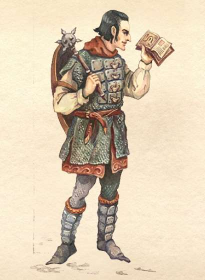
\includegraphics[width=0.45\textwidth]{Pilgrim.png}}
\end{figure}

\begin{figure}[H]
\floatbox[{\capbeside\thisfloatsetup{capbesideposition={right,top},capbesidewidth=0.5\textwidth}}]{figure}[\FBwidth]
{\caption*{Rogue\\

They use speed in combat rather than brute force. Persuasive in conversation, their tongues are as sharp as blades.\\

Specialization: Combat.\\

Attributes: Personality, Speed.\\

Skills: Alchemy, Athletics, Blade, Block, Illusion, Light Armor, Mercantile.}\label{fig:test}}
{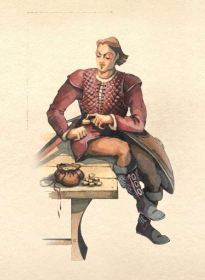
\includegraphics[width=0.45\textwidth]{Rogue.png}}
\end{figure}

\begin{figure}[H]
\floatbox[{\capbeside\thisfloatsetup{capbesideposition={right,top},capbesidewidth=0.5\textwidth}}]{figure}[\FBwidth]
{\caption*{Scout\\

Preferring the rolling countryside to the city life, they are gifted with the ability to evade, guard and protect themselves with great proficiency.\\

Specialization: Combat.\\

Attributes: Endurance, Speed.\\

Skills: Acrobatics, Alchemy, Armorer, Athletics, Blade, Block, Light Armor.}\label{fig:test}}
{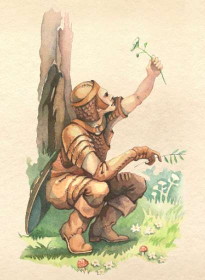
\includegraphics[width=0.45\textwidth]{Scout.png}}
\end{figure}

\begin{figure}[H]
\floatbox[{\capbeside\thisfloatsetup{capbesideposition={right,top},capbesidewidth=0.5\textwidth}}]{figure}[\FBwidth]
{\caption*{Sorcerer\\

Besting the most well-equipped fighters, they rely on the spells of the mystic arts. Unique to these mages is the bodily stamina to be armed with the thickest armor.\\

Specialization: Magic.\\

Attributes: Endurance, Intelligence.\\

Skills: Alchemy, Alteration, Conjuration, Destruction, Heavy Armor, Mysticism, Restoration.}\label{fig:test}}
{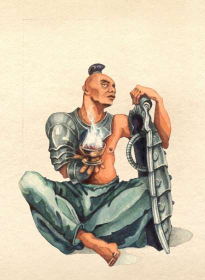
\includegraphics[width=0.45\textwidth]{Sorcerer.png}}
\end{figure}

\begin{figure}[H]
\floatbox[{\capbeside\thisfloatsetup{capbesideposition={right,top},capbesidewidth=0.5\textwidth}}]{figure}[\FBwidth]
{\caption*{Spellsword\\

More nimble and athletic than the sorcerer, and better suited for spell-casting than the knight, their attacks are unpredictable. Students of combat and magic.\\

Specialization: Magic.\\

Attributes: Endurance, Willpower.\\

Skills: Alteration, Blade, Block, Heavy Armor, Destruction, Illusion, Restoration.}\label{fig:test}}
{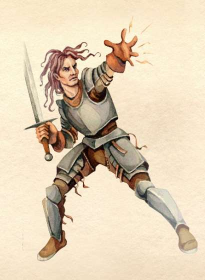
\includegraphics[width=0.45\textwidth]{Spellsword.png}}
\end{figure}

\begin{figure}[H]
\floatbox[{\capbeside\thisfloatsetup{capbesideposition={right,top},capbesidewidth=0.5\textwidth}}]{figure}[\FBwidth]
{\caption*{Thief\\

Profiting from the losses of others is their love. Able to be swift in shadow, and crafty in bartering. Locks are enemies, and lock-picks are their swords.\\

Specialization: Stealth.\\

Attributes: Agility, Speed.\\

Skills: Acrobatics, Light Armor, Marksman, Mercantile, Security, Sneak, Speechcraft.}\label{fig:test}}
{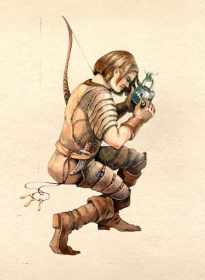
\includegraphics[width=0.45\textwidth]{Thiefclass.png}}
\end{figure}

\begin{figure}[H]
\floatbox[{\capbeside\thisfloatsetup{capbesideposition={right,top},capbesidewidth=0.5\textwidth}}]{figure}[\FBwidth]
{\caption*{Warrior\\

Unafraid of light weaponry, they plow into the fray with little regard for injury. Masters of all melee tools, they put little faith in the magical arts.\\

Specialization: Combat.\\

Attributes: Endurance, Strength.\\

Skills: Armorer, Athletics, Blade, Block, Blunt, Hand-to-Hand, Heavy Armor.}\label{fig:test}}
{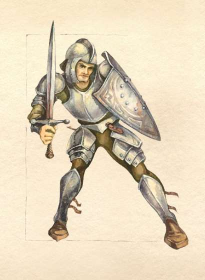
\includegraphics[width=0.45\textwidth]{Warriorclass.png}}
\end{figure}

\begin{figure}[H]
\floatbox[{\capbeside\thisfloatsetup{capbesideposition={right,top},capbesidewidth=0.5\textwidth}}]{figure}[\FBwidth]
{\caption*{Witchhunter\\

Swift on foot, and clever with spells, they use distance as their ally. Slower adversaries are fodder for their arrows.\\

Specialization: Magic.\\

Attributes: Agility, Intelligence.\\

Skills: Alchemy, Athletics, Conjuration, Destruction, Marksman, Mysticism, Security.}\label{fig:test}}
{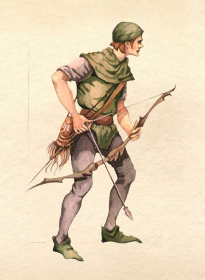
\includegraphics[width=0.45\textwidth]{Witchhunter.png}}
\end{figure}

\newpage
\section{Derive Attributes.}
Now is the time to calculate your derived attributes. There are a lot of things to keep track of here. Be sure to write them down so you don't have to do equations in your head all the time throughout gameplay.
\begin{itemize}
	\item $Health=2*Endurance$.
	\item $Magicka=2*Intelligence$.
	\item $Stamina=Strength+Willpower+Agility+Endurance$.
	\item You recover $(5+0.1Willpower)\%$ of your magicka per round.
	\item You recover 30 stamina per round. This rate increases with Athletics skill (see \textit{Chapter 2: Skills}.)
	\item Your spell range is equal to your Willpower in feet. 
	\item Your movement and damage bonuses are given by the following table.
\end{itemize}

\begin{tabularx}{\textwidth}{|X|X|X|X|X|X|}
\hline
Attribute & 1--24 & 25--49 & 50--74 & 74--99 & 100\\ \hline
Strength & +0 melee & +1 melee & +2 melee & +3 melee & +4 melee\\ \hline
Agility & +0 ranged & +1 ranged & +2 ranged & +3 ranged & +4 ranged\\ \hline
Speed & 20 ft & 30 ft & 40 ft & 50 ft & 60 ft\\ \hline

\end{tabularx}\\~\\

\section{Calculate Skill Points.}
By now, you should have all the information you need to finalize your skill points. The base value of any given skill is 5, so be sure to add all relevant bonuses to that. For example, a Breton Mage begins with a Conjuration of 5(base)+10(racial)+5(magic class)+20(major skill)=40. To learn more about what exactly the skills do, move on to chapter 2. In any case, your character is now complete! Congratulations!

\chapter{Skills}

There are 21 skills in the Elder Scrolls Tabletop RPG. Each one comes with a specialization (combat, magic or stealth), a governing attribute (contributes to attribute increases when you level up), and a set of mastery perks you get automatically when you reach certain skill levels. In addition to providing mastery perks, skill levels determine your proficiency with using the skill and may provide some bonuses such as spell cost reduction. Thus, it's worth boosting stats even if you don't get the next mastery perk. These bonuses will be covered in their respective chapters. In this chapter, you'll find a list of all the skills along with their specializations, governing attributes, meanings and mastery perks.

\section{Skill List}

\begin{tabular}{p{0.2\textwidth}|p{0.2\textwidth}|p{0.15\textwidth}|p{0.45\textwidth}}

Skill & Specialization & Attribute & Uses\\ \hline
Acrobatics & Stealth & Speed & Jumping, climbing and dodging.\\ \hline
Alchemy & Magic & Intelligence & Crafting potions and poisons.\\ \hline
Alteration & Magic & Willpower & Casting spells to change physical properties.\\ \hline
Armorer & Combat & Endurance & Repairing and crafting equipment.\\ \hline
Athletics & Combat & Speed & Sprinting, swimming and stamina recovery.\\ \hline
Blade & Combat & Strength & Attacking with bladed weapons.\\ \hline
Block & Combat & Endurance & Blocking attacks with weapons and shields.\\ \hline
Blunt & Combat & Strength & Attacking with blunt weapons.\\ \hline
Conjuration & Magic & Intelligence & Conjuring minions and equipment from Oblivion.\\ \hline
Destruction & Magic & Willpower & Casting spells to harm foes directly.\\ \hline
Hand-to-Hand & Combat & Strength & Attacking with fists.\\ \hline
Heavy Armor & Combat & Endurance & Effectively using heavy armor.\\ \hline
Illusion & Magic & Personality & Magically manipulating sense and emotion.\\ \hline
Light Armor & Stealth & Speed & Effectively using light armor.\\ \hline
Marksman & Stealth & Agility & Attacking with ranged weapons.\\ \hline
Mercantile & Stealth & Personality & Haggling.\\ \hline
Mysticism & Magic & Intelligence & Casting Mysticism spells.\\ \hline
Restoration & Magic & Willpower & Fortifying stats and healing.\\ \hline
Security & Stealth & Agility & Bypassing locks and other security.\\ \hline
Sneak & Stealth & Agility & Moving silently and striking unseen.\\ \hline
Speechcraft & Stealth & Personality & Speaking persuasively.\\
\end{tabular}

\newpage
\section{Mastery Perks}

Skill levels are grouped into five tiers: Novice (0-24), Apprentice (25-49), Journeyman (50-74), Expert (75-99) and Master (100). Upon achieving each tier, you gain access to a special mastery perk. The following table lists each skill's mastery perks.\\

\begin{tabular}{p{0.15\textwidth}|p{0.12\textwidth}|p{0.15\textwidth}|p{0.15\textwidth}|p{0.13\textwidth}|p{0.15\textwidth}}

Skill & Novice & Apprentice & Journeyman & Expert & Master\\ \hline
Acrobatics & You can attempt to dodge melee attacks for 10 stamina. & Dodging no longer costs stamina. & Non-dodge acrobatics checks in combat cost 30 feet of movement instead of an action. & Non-dodge acrobatics checks in combat cost 15 feet of movement. & Penalty dice due to consecutive dodges are only imposed beginning on your third dodge of the round.\\ \hline
Alchemy & You know the first effect of alchemical reagents. & You know the first two effects of alchemical reagents. & You know the first three effects of alchemical reagents. & You know all effects of alchemical reagents. & You can create potions from single ingredients.\\ \hline
Alteration & Novice Alteration spells. & Apprentice Alteration spells. & Journeyman Alteration spells. & Expert Alteration spells. & Master Alteration spells.\\ \hline
Armorer & PLACEHOLDER & PLACEHOLDER & PLACEHOLDER & PLACEHOLDER & PLACEHOLDER\\

\end{tabular}

\begin{tabular}{p{0.15\textwidth}|p{0.12\textwidth}|p{0.15\textwidth}|p{0.15\textwidth}|p{0.13\textwidth}|p{0.15\textwidth}}

Skill & Novice & Apprentice & Journeyman & Expert & Master\\ \hline
Athletics & Can sprint for double movement (30 stamina, action). & Your swim speed is equal to half your normal movement. & Stamina recovers 40 points per round. & Stamina recovers 50 points per round. & Stamina recovers 60 points per round.\\ \hline
Blade & Blade technique: Power Attack & Blade technique: Standing Strike & Blade Technique: Flanking Strike & Blade Technique: Sweeping Attack & Blade Technique: Dizzying Blow\\ \hline
Block & You can attempt to block melee attacks for 10 stamina. & Blocking no longer costs stamina. & On an extreme success, the attacker suffers recoil. & On a success, 5\% chance of disarming attacker.\\ \hline
Blunt & Blunt technique: Power Attack & Blunt technique: Standing Strike & Blunt Technique: Flanking Strike & Blunt Technique: Sweeping Attack & Blunt Technique: Dizzying Blow\\ \hline
Conjuration & Novice Conjuration spells. & Apprentice Conjuration spells. & Journeyman Conjuration spells. & Expert Conjuration spells. & Master Conjuration spells.\\ \hline
Destruction & Novice Destruction spells. & Apprentice Destruction spells. & Journeyman Destruction spells. & Expert Destruction spells. & Master Destruction spells.\\ \hline
Hand-to-Hand & Unarmed technique: Power Attack & Unarmed technique II & Unarmed technique III & Unarmed technique IV & Unarmed technique V\\

\end{tabular}

\begin{tabular}{p{0.15\textwidth}|p{0.12\textwidth}|p{0.15\textwidth}|p{0.15\textwidth}|p{0.13\textwidth}|p{0.15\textwidth}}

Skill & Novice & Apprentice & Journeyman & Expert & Master\\ \hline
Heavy Armor & You can wear heavy armor. & Heavy armor no longer imposes penalty on Marksman rolls. & Heavy armor movement penalty is reduced by 5 ft. & Heavy armor movement penalty is reduced by 10 ft. & Heavy armor no longer imposes a movement penalty.\\ \hline
Illusion & Novice illusions. & Apprentice illusions. & Journeyman illusions. & Expert illusions. & Master illusions.\\ \hline
Light Armor & You can wear light armor. & ??? & Light armor movement penalty is reduced by 5 ft. & Light armor no longer imposes movement penalty. & Light armor weighs nothing when worn.\\ \hline
Marksman & Archery technique I & archery technique II & archery technique III & archery technique IV & archery technique V\\ \hline
Mercantile & You can buy and sell goods. & You can invest 500 gold into a shop; investment permanently makes the vendor a fence for stolen goods. & You can sell any type of item to any vendor. & Invested shops permanently have an additional 500 gold available for bartering. & All shops have an additional 500 gold available for bartering (stacks with expert).\\ \hline
Mysticism & Novice Mysticism spells. & Apprentice Mysticism spells. & Journeyman Mysticism spells. & Expert Mysticism spells. & Master Mysticism spells.\\

\end{tabular}

\begin{tabular}{p{0.15\textwidth}|p{0.12\textwidth}|p{0.15\textwidth}|p{0.15\textwidth}|p{0.13\textwidth}|p{0.15\textwidth}}

Skill & Novice & Apprentice & Journeyman & Expert & Master\\ \hline
Restoration & Novice Restoration spells. & Apprentice Restoration spells. & Journeyman Restoration spells. & Expert Restoration spells. & Master Restoration spells.\\ \hline
Security & Can pick Very Easy locks. & Can pick Easy locks. & Can pick Average locks. & Can pick Hard locks. & Can pick Very Hard locks.\\ \hline
Sneak & Ranged sneak attacks deal double damage; one-handed sneak attacks deal quadruple damage. & Ranged sneak attacks deal triple damage; one-handed sneak attacks deal 6x damage. & Dagger sneak attacks deal 8x damage. & You may move your full movement while sneaking. & Sneak attacks ignore armor.\\ \hline
Speechcraft & Can bribe NPCs to increase disposition. & Can attempt 4 Speechcraft checks in the same conversation. & Disposition losses from failures are halved. & Bribes cost half as much. & Once per day, guarantee an extreme success on a single check.\\

\end{tabular}

\chapter{Equipment}

\end{document}